% Charlotte Geiger - Manuel Lippert - Leonard Schatt
% Physikalisches Praktikum

% 3.Kapitel  Protokoll

% Variables
\def\skalierung{0.65}

\chapter{Messprotokoll}
\label{chap:protokoll}

Das Messprotokoll wurde am Versuchstag handschriftlich erstellt und hier als
PDF-Datei eingefügt. Dabei wird die Dimensionierung (Datenblatt \footnote{\url{https://docs-emea.rs-online.com/webdocs/0109/0900766b80109ff9.pdf}}) und die gemessenen Widerstände nach dem eigentlichen Messprotokoll eingefügt.\\\\
\textbf{Zusatz:}\\
Da die Bilder der Steckbretter und des Oszilloskops im Protokoll schlecht zu erkennen sind, werden noch zusätzlich die Bilder und angefertigt Schaltpläne der Steckbretter noch angefügt. Es ist noch anzumerken, dass uns beim Ausdrucken der Bilder für (2.2) zwei Bilder (für Messwerte $0.05~mA~\text{und}~0~mA$) vergessen wurden, welche nun im Zusatz nachgereicht werden.

% Einbindung des Protokolls als pdf (mit Seitenzahl etc.)
% Erste Seite mit Überschrift
%\includepdf[pages = 1, landscape = false, nup = 1x1, scale = \skalierung , ]
%            {03 Protokoll/Protokoll.pdf}
% Restliche Seiten richtig skaliert
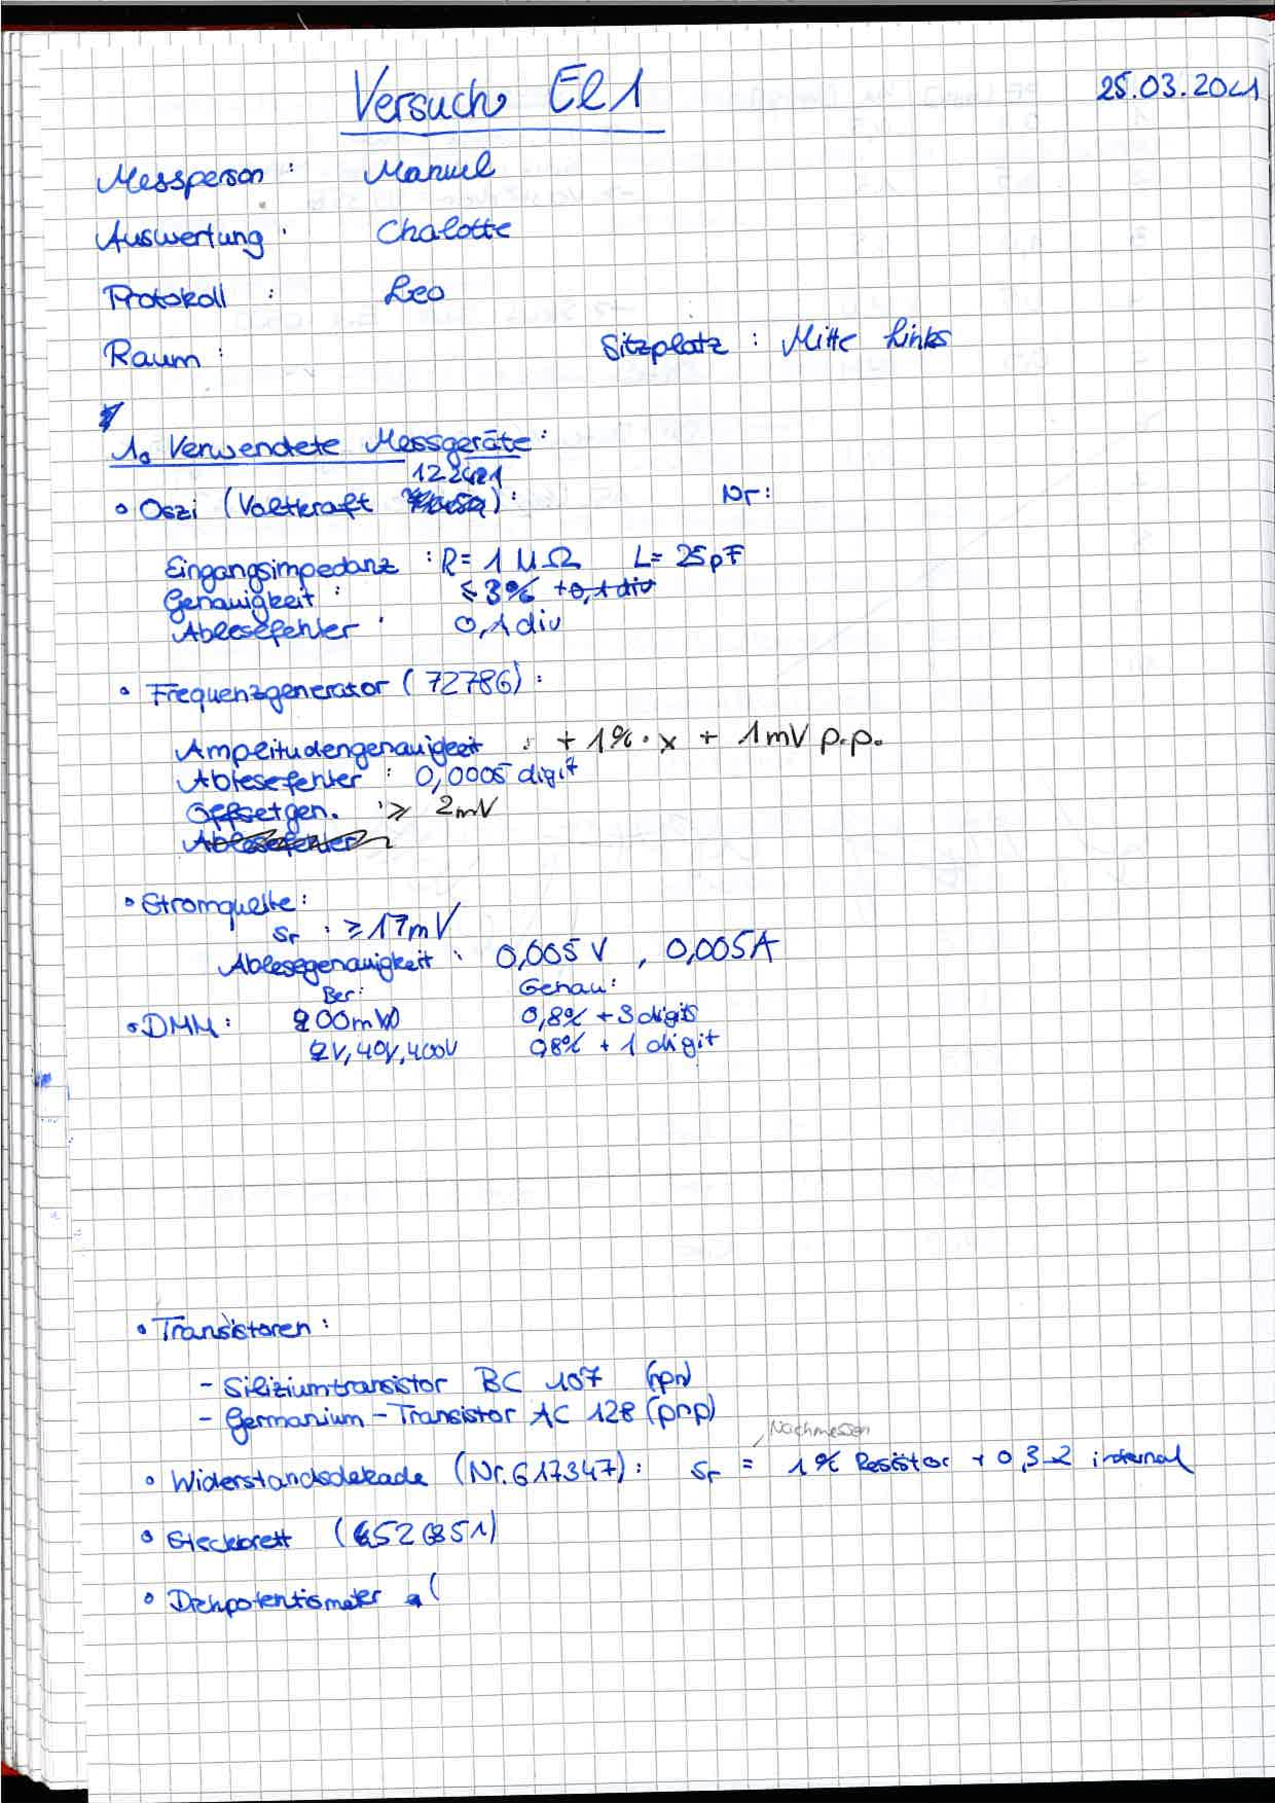
\includepdf[pages = -, landscape = false, nup = 1x1, scale = \skalierung , pagecommand={}]
{03-Protokoll/Protokoll_EL1.pdf}
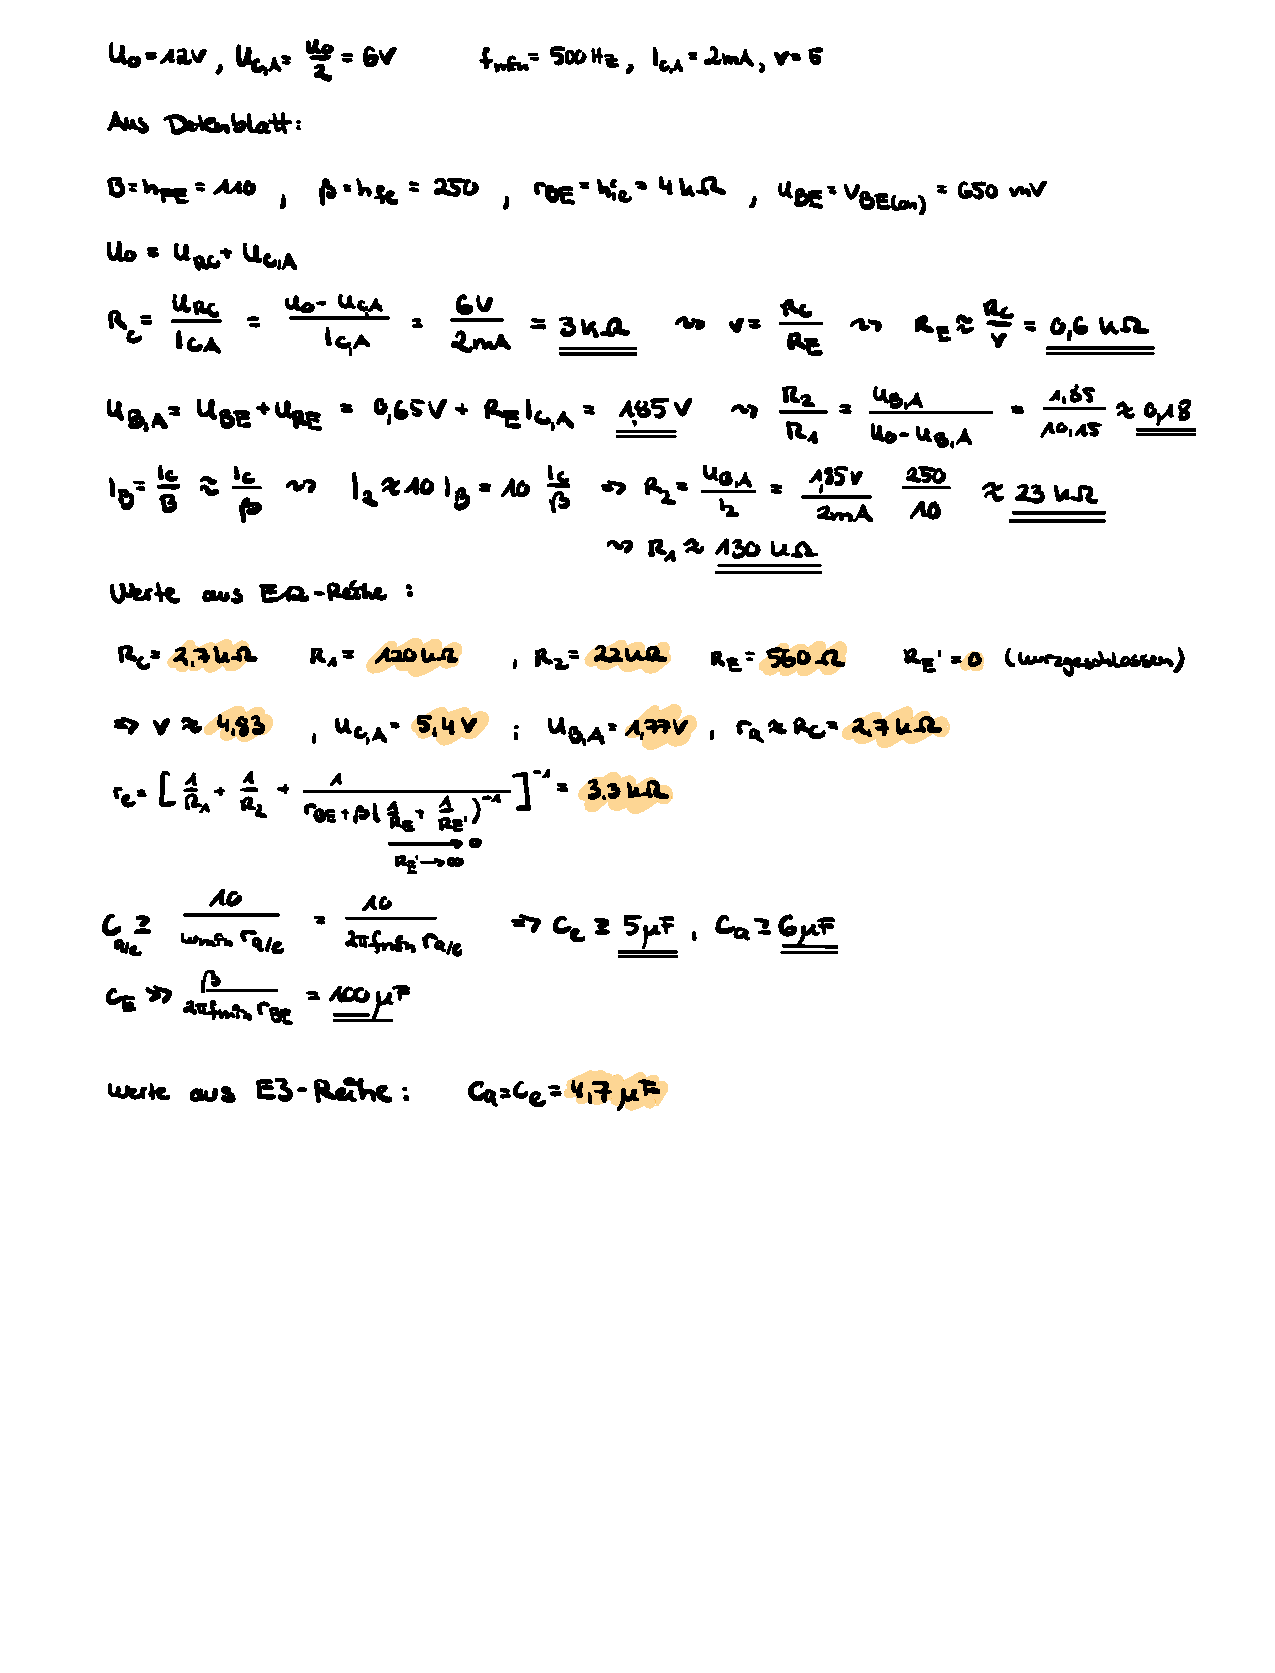
\includepdf[pages = -, landscape = false, nup = 1x1, scale = 0.75 , pagecommand={\section*{Dimensionierung}}]           {03-Protokoll/Dimensionierung.pdf}
\label{sec:zusatz}
\includepdf[pages = 1-2, landscape = false, nup = 1x1, scale = 0.75 , pagecommand={\section*{Zusatz}}]           {03-Protokoll/Bilder_EL1.pdf}
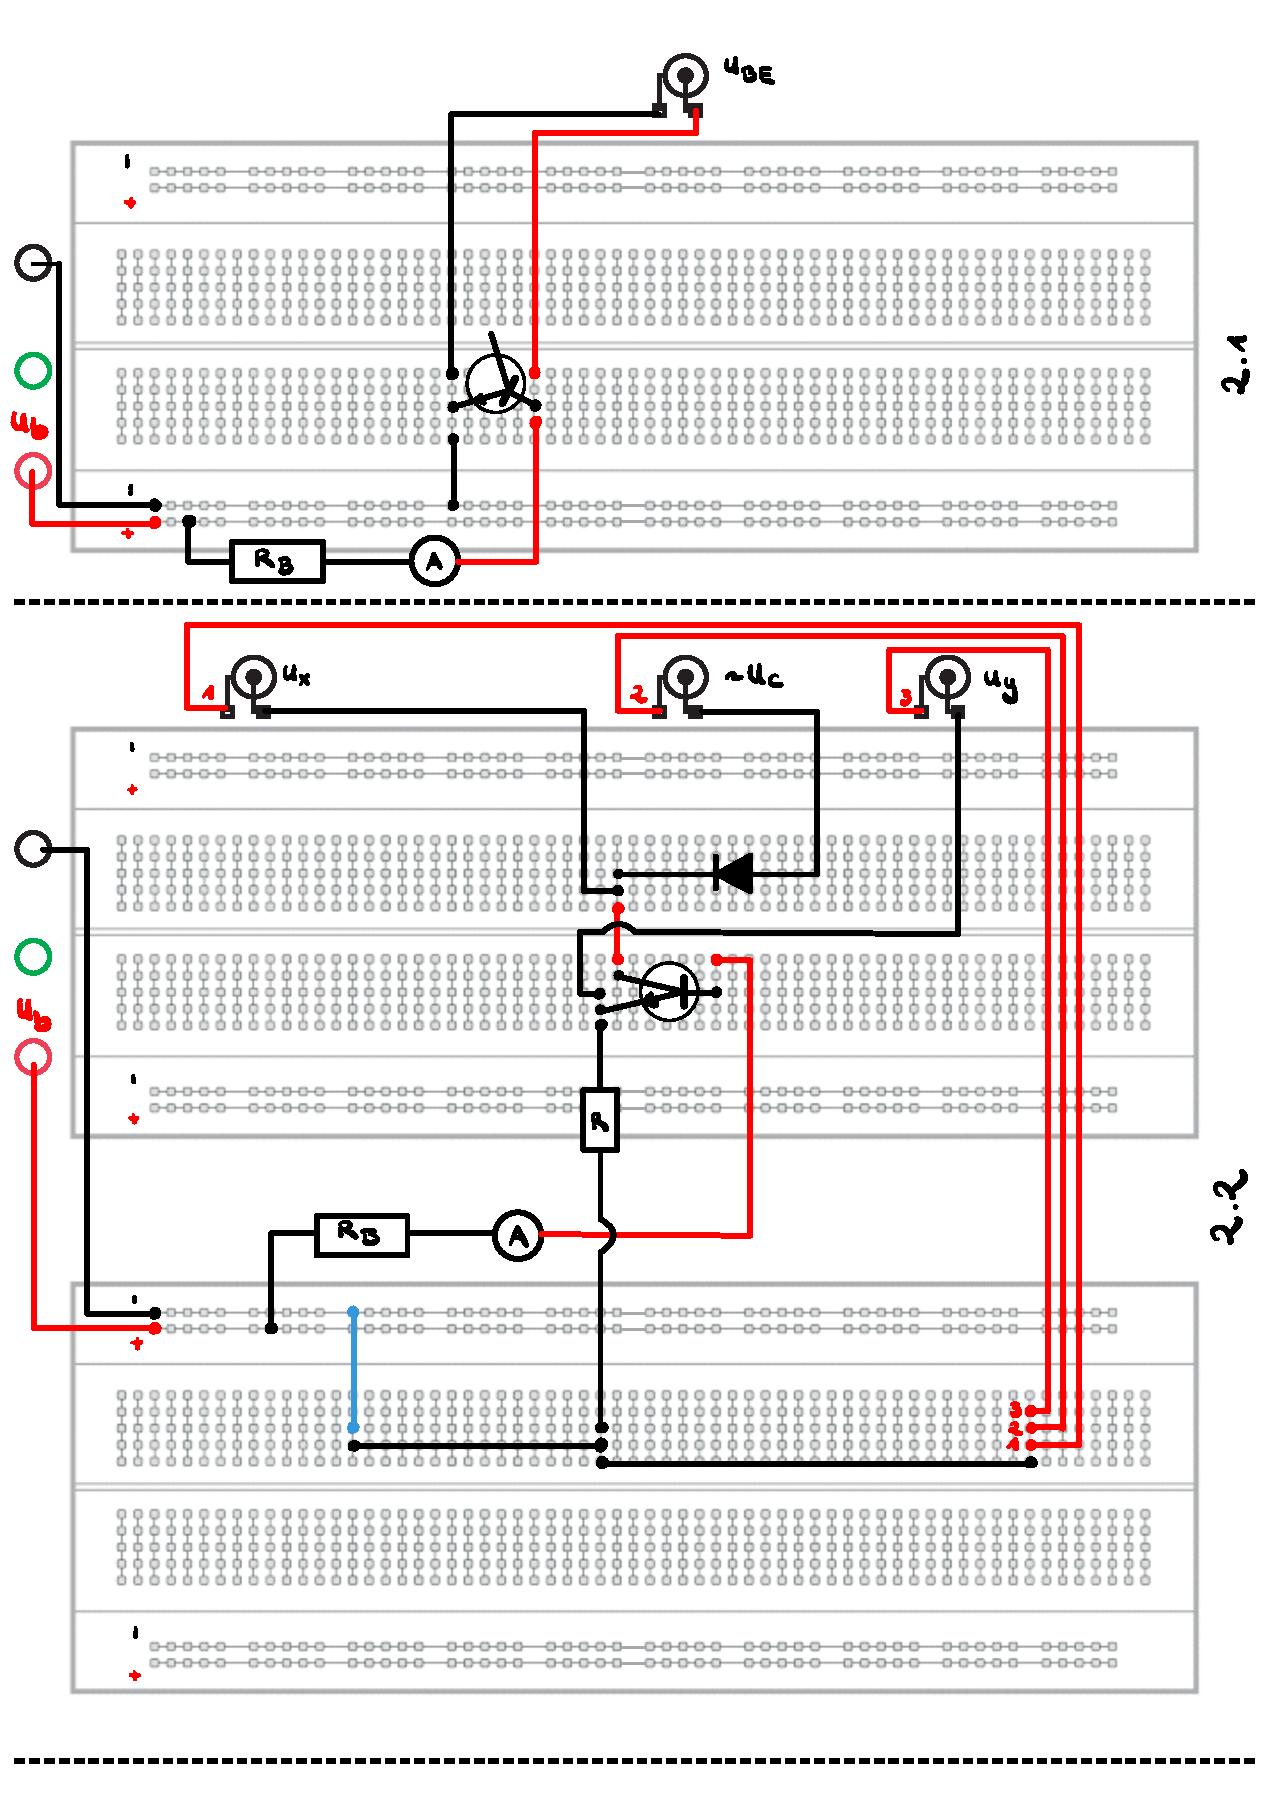
\includepdf[pages = -, landscape = false, nup = 1x1, scale = 0.75 , pagecommand={}]
{03-Protokoll/Steckbretter.pdf}
